\chapter{Progress Report} % Main chapter title

\label{chapter1} % For referencing the chapter elsewhere, use \ref{Chapter1}

%----------------------------------------------------------------------------------------
\section{Introduction}
This capstone project is a study of the principle of self-interpretation, where the aim is to design and implement a self-interpreter for the Scheme programming language, i.e. a Scheme interpreter written in Scheme. 
Scheme was chosen to be the programming language that the self-interpreter will be written in due to its expressive power and minimalism, which will allow us to better explore the principles of self-interpretation. 
The purpose behind the implementation of such a self-interpreter is to explore the richness of the expressivity of the programming language used, and to also study the computational aspects of such self-interpreters, 
e.g. its efficiency. 
\\
\\
Once the implementation of the self-interpreter in Scheme is complete, we will be able to measure the computational cost of layering software 
(e.g. a processor running a virtual machine running a simulator running yet another virtual machine and so on...) in the idealized setting where all the levels of the software are identical 
(Scheme and its self-interpreters, or a tower of Scheme self-interpreters). Furthermore, we can also measure the additional costs incurred due to Scheme’s non-static typing such as the type-checking of each 
argument done in the implementation of the self-interpreter, via implementing a self-interpreter that assumes that all its input is of the correct type and comparing this with one that does the necessary type checks.

\section{Why write a Scheme interpreter in OCaml first?}
Before starting on the implementation of the Scheme self-interpreter, I first started on the implementation of an interpreter for Scheme written in OCaml first. 
This additional step is done for an easier implementation of the self-interpreter for Scheme, where instead of implementing the Scheme self-interpreter from scratch, we will have a reference (and working) interpreter for Scheme 
written in OCaml, which can then be used for transliteration to implement the Scheme self-interpreter.
\\
\\
OCaml was chosen as the metalanguage of the initial interpreter for Scheme, due to my familiarity of with the language as well as the following important characteristics of OCaml:
\begin{enumerate}
   \item Static-typing: OCaml’s nature of being statically-typed is greatly useful in the implementation of an interpreter that is \textit{guaranteed} to be free from \textbf{type-errors}, which can be a real nuisance and creep in 
   as run-time errors if the metalanguage for the interpreter was a language that is dynamically typed instead. 
   \item Pattern Matching: OCaml’s ability to do \textit{pattern matching} on otherwise complicated data types can be said to be a blessing for interpreter/compiler writers. The ability to completely de-structure a data type into its constituent constructors allows us to have a 
   high level of \textit{control} over the manipulation of data types, where we get to perform different actions for different constructors for a \textit{single data type}. This is a convenience as compared to the need to implement
   data accesors, where we will first have to use a data predicate to check whether the data is of a specific type, before using the data accessor to fetch the value of the data itself.
   \item Easy recursion over tree-structured datatypes: This is a consequence of OCaml’s ability to do pattern matching over datatypes and allows for the writing of recursive functions over datatypes to be simple and 
   straightforward.
\end{enumerate}
The implementation of an interpreter for Scheme in OCaml will require the following ingredients:
\begin{enumerate}
   \item Implementation of the Grammar of Scheme in OCaml via constructing our own types,
   \item Implementation of the expressible values of the Scheme language, or the possible types that evaluated Scheme programs can take,
   \item Implementation of the \textit{environment}, which stores the definition of variables and allows for the user to re-use the values of these stored variables via the invocation of these variables’ names,
   \item Implementation of \textit{primitive} functions, which are functions that exist as native built-in functions inside the environment that can be used by the user,
   \item Implementation of the interpreter, which recursively evaluates parsed Scheme programs into its result,
   \item Implementation of unit tests, which rigorously tests for each of the above parts to ensure that the interpreter is working as expected.
\end{enumerate}
The following sections then go on to explain the implementation of each of the above 6 parts.

\pagebreak
\section{Grammar of Scheme and Expressions}
\subsection{BNF of Scheme}
The following figure illustrates the \textbf{simplified} grammar of Scheme, written in \textit{BNF}, where the use of Kleene stars and pluses have been operationalized:
\\
\begin{figure}[!h]
  \centering
    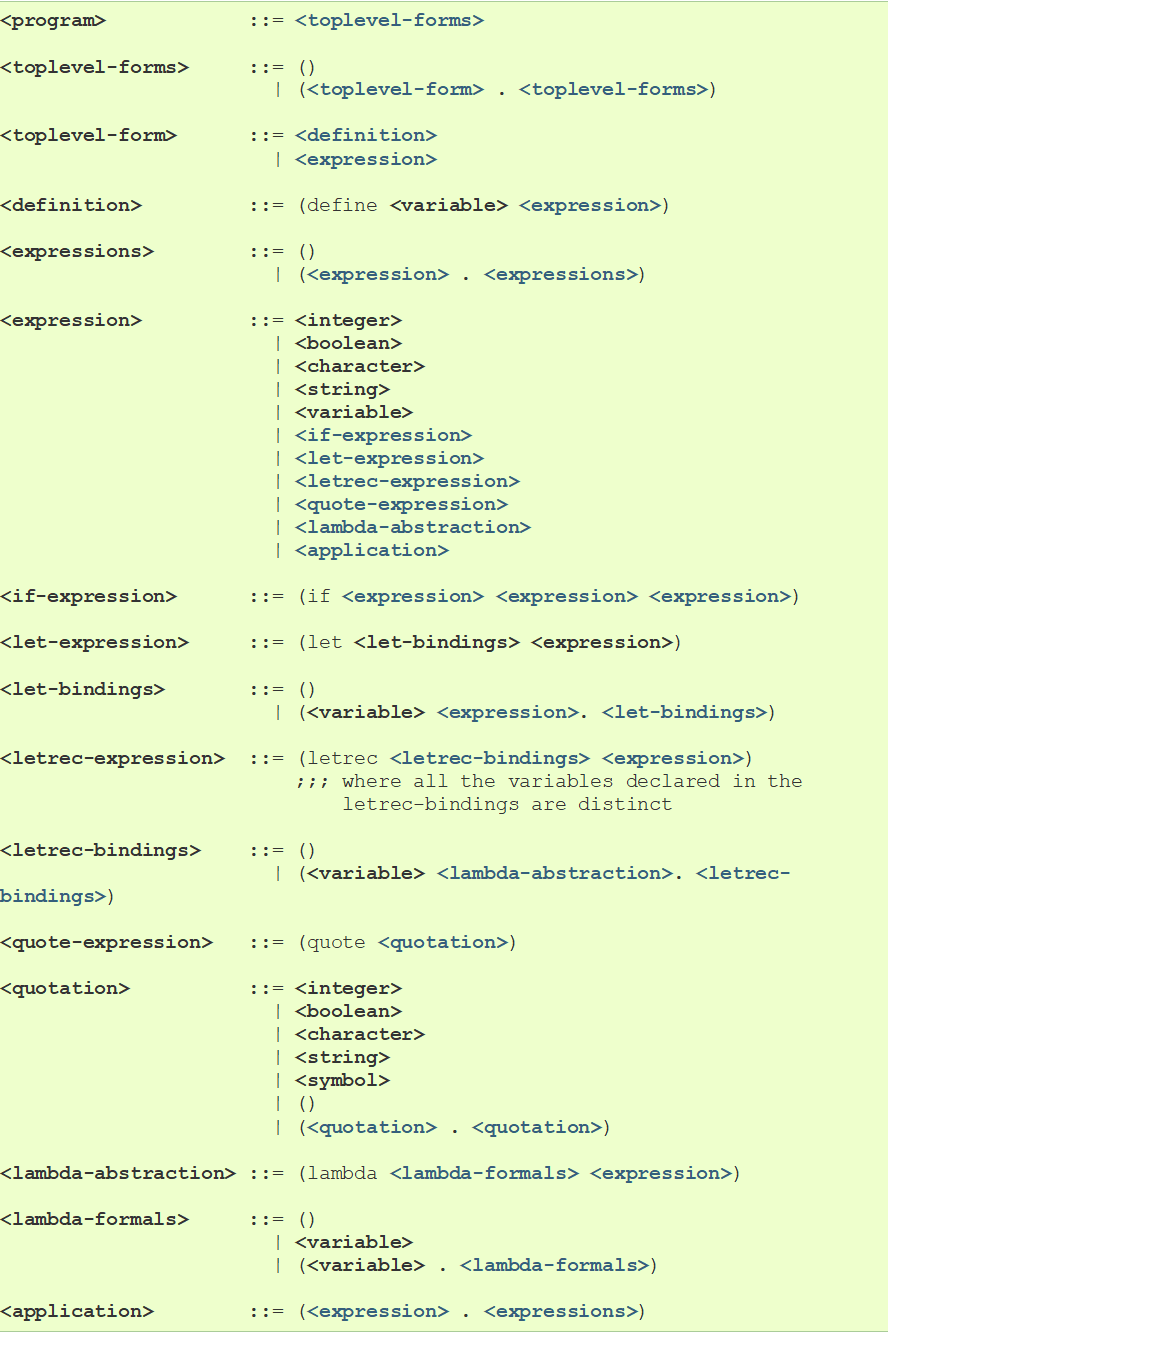
\includegraphics[width=0.9\textwidth]{figures_progress_report/bnf.png}
  \caption{Figure of the operationalized BNF of Scheme}
  \label{fig:bnf}
\end{figure}
\\
The above BNF of Scheme removes some often-seen constructs from Scheme like the and-expression, or-expression, cond-expression, case-expression etc, because the aforementioned constructs are simply syntactic sugar provided by Scheme 
that can be expressed via the use of the if-expression in Scheme. This removal of syntactic sugar constructs allows for the implementation of an interpreter for a smaller yet still complete version of Scheme, which is essential 
given that we only want to focus on the core features of Scheme for the implementation of the interpreter.
\\
\\
The implementation of the operationalized and simplified BNF in OCaml is then as follows, where the quotation type has been left out for now:
\begin{figure}[!h]
  \centering
    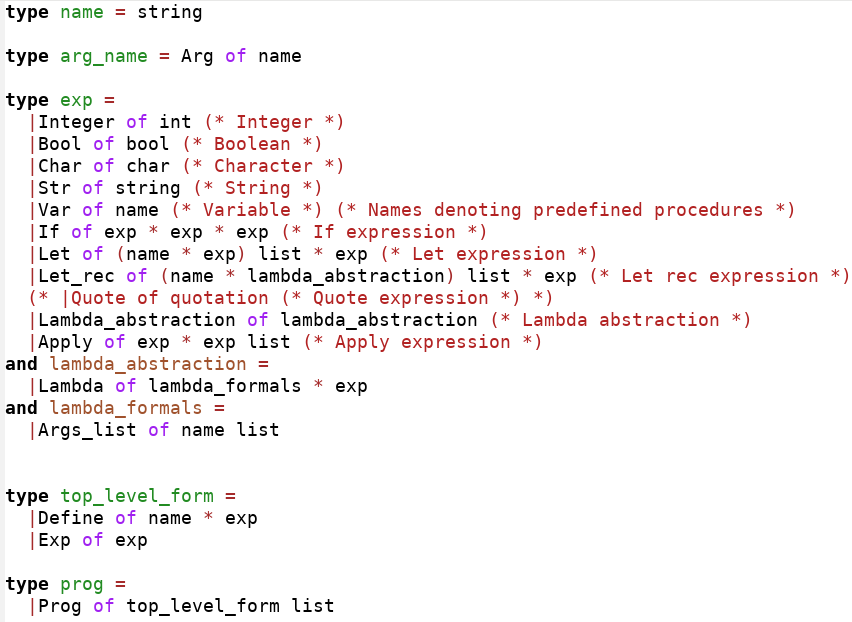
\includegraphics[width=0.9\textwidth]{figures_progress_report/scheme_types.png}
  \caption{BNF of Scheme expressed in OCaml.}
  \label{fig:scheme_types}
\end{figure}

\subsection{Expressible Values}
With the above BNF of Scheme defined in OCaml, we can then proceed to define the various types of expressible values, or the possible types of results we can get via interpreting Scheme programs, as follows:
\begin{figure}[!h]
  \centering
    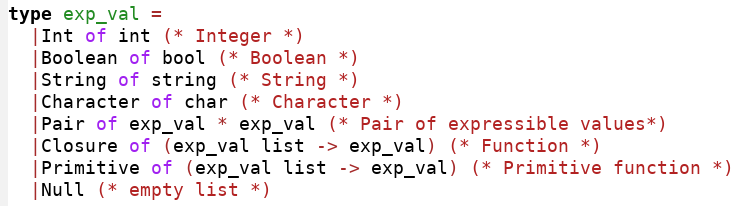
\includegraphics[width=0.9\textwidth]{figures_progress_report/expressible_values.png}
  \caption{Expressible values expressed in OCaml}
  \label{fig:expressible_values}
\end{figure}
\\
Note that in the above definition of expressible values, there exist two types of functions, namely Closures and Primitives. Closures refer to any generic function defined by the user in Scheme, whilst Primitives refer to 
pre-defined functions that exist in the \texitit{environment} of Scheme that can be used by the user without redefinitions. Such pre-defined functions include common operators over integers, Booleans, pairs and the other types of 
expressible values.
\\
\\
We note that the definition of our String and Pair expressible values are immutable in this case, which prevents the use of set! Functions that mutate the values of the string or pair, unlike the original String and Pair values in 
Scheme which are mutable via the set! operation defined in Scheme. This choice of immutability for our Pair expressible values is for the prevention of circularly defined lists, which will require additional cumbersome checks in 
the definition of list-length functions; whilst the choice of immutability for our String expressible values is for consistency (i.e., the use of immutable values for all expressible values) and due to the lack of necessity in 
implementing mutable Strings for the interpreter to work.
\\
\\
We further note that because Lists in Scheme are constructed via the use of Pairs, we have also left out the List type of expressible value since it is expressed via Pairs in Scheme. A \textit{list} in Scheme is defined to be either 
the empty list, or the defined Null value; or a Pair whose cdr is a list. A \textbf{proper} \textit{list} in Scheme is a list that has the empty list as its final element, whilst an \textbf{improper} \textit{list} in Scheme is 
instead a list where the final element is \textbf{not} the empty list. This distinction between proper and improper lists will matter later when we implement our Primitive functions for lists, where the list-length and list-ref functions 
will check for whether the input list is proper or improper before returning a result or an error message.
\\
\\
The remaining types of expressible values, like integers, strings, characters, booleans and the empty list denoted by Null are straightforward in their implementation.

\section{Environment and its related functions.}
As seen from the above defined grammar of Scheme, Scheme supports the use of \textit{variables}, which are essentially named denotations of evaluated Scheme expressions or expressible values. For our interpreter to be able to \
keep track of names and the expressible values they denote, we require the use of an \textit{environment}, which is some sort of memory that keeps track of these name-value pairs. 
\\
\\
In our implementation of the interpreter, we choose to use a simple association list (or a list of pairs), where the first element of the pair stores the name of the variable with the second element of the pair storing the 
expressible value denoted by the name. The type of our environment is then simply:
\begin{small}
\begin{verbatim}
type env = (name * exp_val) list
\end{verbatim}
\end{small}
\\
Our empty environment can then simply be defined as the empty list:
\begin{small}
\begin{verbatim}
let empty_alist = []
\end{verbatim}
\end{small}
With the environment defined, we can then define functions that serve to:
\begin{enumerate}
   \item \textit{Extend} the environment, or adding name-value pairs into the environment,
   \item \textit{Lookup} for the denotation of a name if it exists inside the environment
\end{enumerate}
\\
\\
The basic function that extends the environment simply takes in the name of the variable and its denotation, and returns an environment that has the pair containing the input name and denotation cons-ed onto the original 
input environment:
\begin{small}
\begin{verbatim}
let extend_alist x d env = (x, d) :: env
\end{verbatim}
\end{small}
Beyond this simple implementation, we can define a function that takes in a list of names and a list of denotations instead which adds each name and denotation from the 2 lists elementwise and cons them into the input environment:
\pagebreak
\begin{scriptsize}
\begin{verbatim}
let extend_alist_star xs_given vs_given env =
  let rec visit xs vs = 
    match xs with
    |[] ->
      begin match vs with
      |[] -> env
      |_ ->
        raise (Error
                 (Printf.sprintf
                    "Arity mismatch, %s  %s"
                    (show_list show_string xs_given)
                    (show_list show_exp_val vs_given)))
      end
    |x :: xs' ->
      begin match vs with
      |[] ->
        raise (Error
                 (Printf.sprintf
                    "Arity mismatch,  %s  %s"
                    (show_list show_string xs_given)
                    (show_list show_exp_val vs_given)))
      |v :: vs' ->
        (x , v) :: visit xs' vs'
      end
  in visit xs_given vs_given
\end{verbatim}
\end{scriptsize}
\\
The above function is recursive in nature and recurses over the list of names, with the inductive specification being as follows:
\begin{enumerate}
   \item Base Case: If the input list of names is the empty list, and if the input list of denotations is also the empty list, we simply return the environment. Otherwise, if the input list of denotations is not the empty list, 
   we raise an error due to the differing lengths of the 2 input lists.
   \item Induction Step: If the input list of names can be represented as x :: xs’, where x is the head of the list and xs’ is the tail of the list, if the input list of denotations is the empty list, we raise an error due to 
   the differing lengths of the 2 input lists. Otherwise, if the input list of denotations can be represented as v :: vs’, where v is the head of the list of denotations and vs’ is the tail of the list of denotations, the result 
   is simply (x, v) cons onto the induction hypothesis, which is the result of the function applied on xs’ and vs’.
\end{enumerate}
\\
For the lookup function, the implementation is simple where we simply recurse over the environment and find the first instance of the pair containing the name and return its corresponding denotation from said pair; otherwise 
if we have recursed through the entire environment and don’t find any matching pairs, we raise the Not\_found error to indicate that the name does not exist in the environment:
\begin{scriptsize}
\begin{verbatim}
let rec lookup (x:name) (c: env) : exp_val =
  begin
    match c with
    |[] ->
      raise Not_found
    |l :: ls' ->
      begin
        match l with
        |(y, z) ->
          if x = y then z
          else lookup x ls'
      end
  end
\end{verbatim}
\end{scriptsize}

\section{Primitive Functions}
With the environment and its functions defined, we can go ahead to define the primitive functions (or in-built functions) of Scheme and initialize these functions inside our initial environment for use. 
The in-built functions for Scheme can be grouped based on:
\begin{enumerate}
   \item The type of \textit{object} the function acts on. Example objects include integers, strings, characters, Booleans, pairs and lists.
   \item The \textit{arity} of the function, i.e., the number of valid arguments the function can take. Some functions have no defined arity and can take in any number of arguments, whilst some functions have fixed arity and are only 
   defined for, as an example, one or more arguments. We further note that in Scheme, procedures (or functions) are \textit{uncurried}, and their arguments are naturally stored in a list. This essentially means that the number of 
   arguments supplied to the function is equal to the number of elements inside the list. Hence, testing whether the number of arguments supplied to the function is correct involves using OCaml’s pattern matching to check 
   for the number of elements in the list storing the arguments.
   \item The type of the function, i.e. whether it is a comparison function, an indexing function, a function that creates an object from multiple other objects etc.
\end{enumerate}
Given the large number of essential primitive functions to define, this section will only elaborate on a representative sample of the primitive functions that we have defined for the interpreter. 
\subsection{Functions that act on Pairs}
An example function that acts on pairs would be the binary function Cons, which takes in two arguments and returns a Pair with the first input argument as its car and the second input argument as its cdr:
\begin{scriptsize}
\begin{verbatim}
let internal_cons =
  (fun vs ->
    begin
      match vs with
      |v1 :: v2 :: [] ->
        Pair (v1, v2)
      |_ ->
        raise (Error
                 (Printf.sprintf
                    "Incorrect argument count in call %s"
                    (show_list show_exp_val vs)))
    end)
\end{verbatim}
\end{scriptsize}
\\
where a suitable error message printing the arguments supplied (via the use of an unparser) if the number of arguments is incorrect is shown.
\\
\\
Another function that is similar but involves type-checking is the car function that returns the first element contained inside the pair:
\begin{scriptsize}
\begin{verbatim}
let internal_car =
  (fun vs ->
    begin
      match vs with
      |v :: [] ->
        begin
          match v with
          |Pair (v1, _) ->
            v1 
          |_ ->
            raise (Error
                     (Printf.sprintf
                        "Error in car: %s is not a pair."
                        (show_exp_val v)))
        end
       
       
      |_ ->
        raise (Error
                 (Printf.sprintf
                    "Incorrect argument count in call %s"
                    (show_list show_exp_val vs)))
    end)
\end{verbatim}
\end{scriptsize}
\\
The car function is unary and is only defined for pairs. Hence, as per its definition in Scheme, the function first checks for whether the number of arguments supplied to it is correct (and printing an error message if the number 
of arguments is incorrect), before checking for the type of argument. If the type of argument is a pair, the function returns the car of the argument; otherwise the function will return an error stating that the supplied 
argument is of an incorrect type, i.e., not a pair, using our pre-defined unparser.
\\
\\
The remaining functions for pairs are like the above two with the only exception being their functionality.
\subsection{Functions that act on Integers}
For integers, most of the functions that act on them are functions that do mathematical operations or comparisons. Hence, although we would expect these functions to only take in 2 arguments, most of them are however 
defined to have no fixed arity (variadic) with only a few of them accepting just 1 or 2 arguments.
\\ 
\\
For this section, we would provide 3 representative functions, namely:
\begin{enumerate}
   \item A function that does mathematical operations which is variadic in nature, 
   \item A function that also does mathematical operations which is binary /dyadic in nature,
   \item A unary function that checks for the nature of the integer argument.
\end{enumerate}
An example of a function that does mathematical operations and is variadic in nature would be the addition function. In Scheme, the addition function is variadic and simply returns the result of adding all its arguments 
if they are all integers or returning an error if any one of them is not an integer. Specifically: 
\begin{enumerate}
   \item For the case where the addition function is supplied with 0 arguments, the addition function simply returns 0, or the \textit{neutral element} of addition, because adding anything with 0 leaves the result unaltered.
   \item If the additon function is supplied with 1 argument (of integer type), the addition function then returns that argument because it is the result of adding 0 and that argument.
   \item If the addition function is supplied with 2 or more arguments (all of integer type), the addition function then returns the result of adding all these arguments together.
\end{enumerate}
\\ 
We can define such a variadic function in OCaml using a \textit{tail-recursive} function that takes in a list of integers as an argument:
\begin{scriptsize}
\begin{verbatim}
let internal_add =
  (fun vs ->
    let rec visit_add vs' a =
      begin
        match vs' with
        |[] ->
          Int a
        |v :: vs'' ->
          begin
            match v with
            |Int i ->
              visit_add vs'' (a + i)
            |_ ->
              raise (Error
                       (Printf.sprintf
                          "Error in +: %s is not a number."
                          (show_exp_val v)))
          end
      end
    in visit_add vs 0)
\end{verbatim}
\end{scriptsize}
\\
The inductive specification of the above addition function is as follows:
\begin{enumerate}
   \item Base Case: When the list of arguments is the empty list (i.e., no arguments are supplied), we simply return the accumulator a which is initialized to be 0 as per the behavior of addition in Scheme.
   \item Induction Step: When the list of arguments can be represented as v :: vs’, we first check whether the element v is of type integer. If v is of type integer and can be represented as Integer i, 
   we know that the result of the function is simply our induction hypothesis visit\_add vs’ initialized with the accumulator as \textit{(a + i)}.
\end{enumerate}
\\
An example of a function that does mathematical operations and is binary / dyadic in nature would be the quotient function. The quotient function simply takes in a list containing 2 integer arguments, and 
returns the quotient that is a result of dividing the first argument by the second argument:
\begin{scriptsize}
\begin{verbatim}
let internal_quotient =
  (fun vs ->
    begin
      match vs with
      |v1 :: v2 :: [] ->
        begin
          match v1 with
          |Int i1 ->
            begin
              match v2 with
              |Int i2 ->
                if i2 = 0
                then raise (Error
                              (Printf.sprintf
                                 "Error in quotient: undefined for 0."))
                else
                  Int (i1 / i2)
              |_ ->
                raise (Error
                         (Printf.sprintf
                            "Error in quotient: %s is not a number."
                            (show_exp_val v2)))
            end
          |_ ->
            raise (Error
                     (Printf.sprintf
                        "Error in quotient: %s is not a number."
                        (show_exp_val v1)))
        end
      |_ ->
        raise (Error
                 (Printf.sprintf
                    "Incorrect argument count in call %s"
                    (show_list show_exp_val vs)))
    end)
\end{verbatim}
\end{scriptsize}
From the above function, we note that the function does a lot of type checking for each of the 2 arguments and returns an error message if either of the 2 arguments is not an integer. We further note the checking of the 
2nd integer argument to see whether it is 0, because the division by 0 error will have to be raised for such a case (which in Scheme will raise the same error message we wrote in the function).
\\
\\
Finally, an example of a unary function that checks for the nature of the integer argument would be the is-even function. The implementation of the is\_even function is simple: If there is only 1 argument supplied and it is of type 
integer, we simply check whether the remainder of dividing said argument by 2 is 0 and return the expressible value Boolean true if it is so and Boolean false otherwise. A wrong number of arguments of a non-integer argument 
will raise an error:
\begin{scriptsize}
\begin{verbatim}
let internal_is_even =
  (fun vs ->
    begin
      match vs with
      |v :: [] ->
        begin
          match v with
          |Int i ->
            if (i mod 2) = 0
            then Boolean true
            else
              Boolean false
          |_ ->
            raise (Error
                     (Printf.sprintf
                        "Error in even?: %s is not a number."
                        (show_exp_val v)))
        end
      |_ ->
        raise (Error
                 (Printf.sprintf
                    "Incorrect argument count in call %s"
                    (show_list show_exp_val vs)))
    end)
\end{verbatim}
\end{scriptsize}
\\
A large bulk of the remaining functions not illustrated here are variadic functions that test whether the integer arguments provided are monotonically increasing, decreasing or are all equal to each other, and are 
implemented recursively as well via the use of an accumulator. An example of a comparison function would be provided in the following section for functions operating on Characters, with the implementation being the 
same modulo the type of object being operated on. 
\\
\\
The remaining binary mathematical operators are implemented similarly to addition, albeit with subtraction and division not allowing for the case of 0 arguments (since there is no neutral element for these operations).
\subsection{Functions that act on Characters}
For characters, most of the functions that act on them are functions that do comparisons between them or check that a character belongs to a certain category. 
\\
\\
For this section, we would provide 2 representative functions, namely:
\begin{enumerate}
   \item A function that does comparisons between characters which is variadic in nature,
   \item A unary function that checks for the type of an input character
\end{enumerate}
\\
An example function that does comparisons would be the lesser than comparison function. The lesser than comparison function checks whether each argument (of type character) is less than the arguments that come after it. 
In other words, the function checks that the arguments it is supplied with are monotonically increasing and requires at least one argument to be supplied.
\\
\\
Such a variadic functionc can be defined using tail-recursion over the list, with the inductive specification being as follows:
\begin{enumerate}
   \item Base Case: In the base case where the list of arguments is empty, we return the accumulator a, which is initialized to be the Boolean value true.
   \item Induction Step: If the list of arguments can be represented as v :: vs’, if v is a character c and is greater than the previous character c’ (stored as another argument of the function), the result of 
   the function would be the same as the induction hypothesis (recursing over the remaining list) with the accumulator being the same, and with c being stored as c’ in the function to be compared with the next 
   argument. Otherwise, if c is not greater than c’, we change the Boolean value stored in the accumulator to false (and do nothing if it is already stored as false) and store c as c’ too, before recursing through 
   the remainder of the list to check whether any incorrect arguments exist in the remainder of the list and raise errors if there are any.
\end{enumerate}
The function is then as follows:
\begin{scriptsize}
\begin{verbatim}
let internal_char_lt =
  (fun vs ->
    begin
      match vs with
      |[] ->
        raise (Error
                 (Printf.sprintf
                    "Incorrect argument count in call %s"
                    (show_list show_exp_val vs)))
      |v1 :: vs' ->
        begin
          match v1 with
          |Character c1 ->
            let rec visit_char_lt vs c' a =
              begin
                match vs with
                |[] ->
                  Boolean a
                |v :: vs' ->
                  begin
                    match v with
                    |Character c ->
                      if c > c'
                      then visit_char_lt vs' c a
                      else
                        if a
                        then visit_char_lt vs' c false
                        else
                          visit_char_lt vs' c a
                    |_ ->
                      raise (Error
                               (Printf.sprintf
                                  "Error in char<?: %s is not a character."
                                  (show_exp_val v)))
                  end
              end
            in visit_char_lt vs' c1 true
          |_ ->
            raise (Error
                     (Printf.sprintf
                        "Error in char<?: %s is not a character."
                        (show_exp_val v1)))
        end
    end)
\end{verbatim}
\end{scriptsize}
\\
where we raise an error indicating an incorrect argument count if no arguments were supplied, and otherwise initialize the tail-recursive function specified above with the Boolean true as its accumulator and the first 
character argument of the list as c’. If any of the input arguments are not of type character, an error message indicating type error is raised. All the comparison functions for the integer and string object types 
work in the same fashion as well.
\\
\\
An example of a unary function that checks whether an input character argument is of a specific group is the is-numeric function, which checks whether the input character is numeric. The implementation of such a function is 
straightforward and simply uses OCaml’s pattern matching:
\begin{scriptsize}
\begin{verbatim}
let internal_char_numeric =
  (fun vs ->
    begin
      match vs with
      |v :: [] ->
        begin
          match v with
          |Character c ->
            begin
              match c with
              |'0' |'1' |'2' |'3' |'4' |'5' |'6' |'7' |'8' |'9' ->
                Boolean true
              |_ ->
                Boolean false
            end
          |_ ->
            raise
              (Error
                 (Printf.sprintf
                    "Error in char-numeric?: %s is not a character."
                    (show_exp_val v)))
        end
      |_ ->
        raise (Error
                 (Printf.sprintf
                    "Incorrect argument count in call %s"
                    (show_list show_exp_val vs)))
    end)
\end{verbatim}
\end{scriptsize}
\\
where as before, errors are raised if the number of arguments is incorrect or if the single input argument is not of type character.
\subsection{Functions that act on Strings}
For the case of strings, most of the its inbuilt functions are comparison type functions, with str-ref and str-length being the few exceptions.  For a representative sample of functions that act on strings, only the 
unary function str-length will be illustrated:
\begin{scriptsize}
\begin{verbatim}
let internal_str_length =   
  (fun vs ->
    begin
      match vs with
      |v :: [] ->
        begin
          match v with
          |String s ->
            let len = String.length s in
            Int len
          |_ ->
            raise (Error
                     (Printf.sprintf
                        "Error in string-length?: %s is not a string."
                        (show_exp_val v)))
        end
      |_ ->
        raise (Error
                 (Printf.sprintf
                    "Incorrect argument count in call %s"
                    (show_list show_exp_val vs)))
    end)
\end{verbatim}
\end{scriptsize}
\\
As seen in the screenshot above, the implementation of str\_length is very straightforward and is mainly implemented by OCaml’s inbuilt String.length function. As is usual for primitive functions, the number of 
arguments and type checking occurs as well, with the appropriate errors being raised if required.
\\
\\
As of now, the in-built functions for the list object has been left out in our initial implementation of the Scheme interpreter written in OCaml and will be implemented later on when we are writing our self-interpreter for Scheme.
\\
\\
With our primitive functions defined, our initial environment of the interpreter is then an association list containing the names of the inbuilt function and their denotations, namely the primitive functions defined.
\section{The Interpreter (eval) Function}
With the primitive functions and the environment now defined, we can proceed to implementing the main interpreter function.
\\
\\
The interpreter is a function that takes in a Scheme expression (parsed Scheme code) and performs the expected behavior of the expression according to the specified grammar of Scheme, before returning an expressible value or 
the result of the computing the Scheme expression. Our interpreter written in OCaml is recursive in nature, and recurses over the AST of the Scheme expressions. The specification for the OCaml interpreter for Scheme is as follows:
\begin{enumerate}
   \item Base Case: If the Scheme expression is: 
   \begin{enumerate}
      \item An integer n: An expressible value of type integer with value n will be returned.
	  \item A Boolean b: An expressible value of type Boolean with value b will be returned.
	  \item A character c: An expressible value of type Character with value c will be returned.
	  \item A string s: An expressible value of type String with value s will be returned.
	  \item A variable x: An expressible value which is the result of looking up x in the current environment will be returned.
   \end{enumerate}
   \item Induction Step: If the Scheme expression is:
   \begin{enumerate}
      \item An if expression \textit{if(e1, e2, e3)}: If the result of interpreting the Scheme expression e1 is not the Boolean false, the result of interpreting the Scheme expression e2 will be returned. 
	  Else, the result of interpreting the Scheme expression e3 will be returned.
	  \item An apply expression \textit{apply(e, es)}: If the result of interpreting the Scheme expression e is a Closure function or a Primitive function, and the result of interpreting the list of Scheme expressions es 
	  is the list of expressible values vs, then the result of the apply expression is simply the application of the Closure/Primitive function on the list of expressible values vs.
	  \item A lambda expression \textit{lambda(formals, body)}: If the formals is simply a list of arguments xs, the result of interpreting the Scheme expression of lambda will be the Closure function that takes in a list of 
	  arguments vs, binds them to the list of arguments xs, and evaluates/interprets the body of the lambda expression in the extended environment containing the bindings of the argument names xs to the arguments in list vs.
   \end{enumerate}
\end{enumerate}
\\
We note that the let and let-rec constructs have not been implemented for the interpreter yet and will be implemented after the submission of this progress report. 
\\
\\
Furthermore, we note that the definition of a helper function will be required for the case where we evaluate the apply expression, or specifically, the list of expressions es in the apply expression. The helper function is simply 
a function that takes in a list of Scheme expressions and returns a list of expressible values which are the result of interpreting the aforementioned Scheme expressions, and its inductive specification is as follows:
\begin{enumerate}
   \item Base Case: If the list of Scheme expressions exps is the empty list, then the result is also the empty list.
   \item Induction Step: If the list of Scheme expressions exps can be represented as exp :: exps’, then the result of the helper function applied on exps is the same as cons-ing the interpreted result of exp onto the result of 
   the helper function applied on exps’ (the induction hypothesis).
\end{enumerate}
With the definition of the interpreter and its helper function complete, the implemented interpreter (and helper function) is as follows:
\pagebreak
\begin{scriptsize}
\begin{verbatim}
let rec eval (exp : exp) (env: env): exp_val =
  begin
    match exp with
    |Integer i ->
      Int i
    |Bool b ->
      Boolean b
    |Var x ->
      lookup x env
    |Str s ->
      String s
    |Char c ->
      Character c
    |If (exp1, exp2, exp3) ->
      begin
        match (eval exp1 env) with
        |Boolean false ->
          eval exp3 env
        |_ ->
          eval exp2 env
      end
    |Apply (e, es) ->
      (* Left to right evaluation order *)
      let v = eval e env in
      let vs = evlis es env in
      begin
        match v with
        |Closure p ->
          p vs
        |Primitive p ->
          p vs
        |_ ->
          raise (Error
                   (Printf.sprintf
                      "Not a procedure: %s"
                      (show_exp_val v)))
      end
    |Let (_, _) ->
      raise Not_implemented_yet
    |Let_rec (_, _) ->
      raise Not_implemented_yet
    |Lambda_abstraction (Lambda(formals, body)) ->
      begin
        match formals with
        |Args_list xs ->
          Closure
            (fun vs ->
              eval
                body
                (extend_alist_star xs vs env))
      end                          
  end
and evlis (exps : exp list)(env : env): exp_val list =
  begin
    match exps with
    |[] ->
      []
    |exp :: exps' ->
      (* To ensure left to right order evaluation *)
      let v = eval exp env
      in v :: evlis exps' env
  end;;
\end{verbatim}
\end{scriptsize}
\\
where we set the evaluation order of the interpreter to be from left to right. This left to right evaluation order can be explicitly seen from what happens in the apply clause of the interpreter and the evlis helper function, 
where we explicitly evaluate the head of the list exps first before evaluating its tail exps’; or when we explicitly evaluate the left argument of the apply expression e before evaluating its right argument es. Not doing 
any one of the above would lead to an interpreter that has an inconsistent order of evaluation, because since OCaml is a programming language that has a right to left order of evaluation, not explicitly evaluating exp 
first before exps’ in the case of evlis, for example, will lead to the case where exps’ is evaluated first before exp instead in the recursive clause where exps can be represented as exp::exps’.
\section{Testing}
With the implementation of the grammar of Scheme, expressible values, the interpreter environment, the primitive functions and the interpreter somewhat completed, we can then proceed to conduct extensive testing for each of 
these components of our interpreter before we proceed to implement trickier cases such as the let-rec case for our interpreter which has been left intentionally incomplete as of now. This is because once we have an error-free 
base interpreter, implementing the let-rec case which handles recursive functions will be much easier as the errors raised are now due to errors in the implementation of let-rec and not due to any other buggy feature of the 
interpreter.
\\
\\
Our testing for the interpreter can then be divided according to the following components:
\begin{enumerate}
   \item The environment and its related functions,
   \item The primitive functions,
   \item The base interpreter as it is.
\end{enumerate}
Furthermore, since we want our testing to satisfy \textit{code coverage}, we not only want to test that our interpreter (and its components) return the correct values when their arguments are error-free, but also want to 
test that they will return the \textit{correct error} when the arguments are erratic (either in terms of type or in terms of the number of arguments).
\\
\\
The tests can be divided into the following two broad categories:
\begin{enumerate}
   \item Testing that the function gives the correct output given that the input arguments are well-typed and are of the correct number.
   \item Testing that the function raises the correct error given either an incorrect type of input argument or an incorrect number of input arguments.
\end{enumerate}
\subsection{Testing the is\_even function for correct output}
Referring to the is\_even function described in the Primitives section above, we can see that to ensure code coverage for the non-error branches, we will have to test for the case where there is only a single argument which is 
of type integer, and test for even and non-even numbers. The following screenshot of the test illustrates the above:
\begin{scriptsize}
\begin{verbatim}
let test_internal_is_even candidate =
  (* Test for the case where input is even *)
  let b0 = (candidate [Int 0] = Boolean true)
  and b1 = (candidate [Int 2] = Boolean true)
  and b2 = (candidate [Int 40296] = Boolean true)
  and b3 = (candidate [Int (-2)] = Boolean true)
  and b4 = (candidate [Int (-20148)] = Boolean true)
  (* Test for the case where input is odd *)
  and b5 = (candidate [Int 1] = Boolean false)
  and b6 = (candidate [Int 3] = Boolean false)
  and b7 = (candidate [Int (-19)] = Boolean false)
  and b8 = (candidate [Int (-20149)] = Boolean false)
  in b0 && b1 && b2 && b3 && b4 && b5 && b6 && b7 && b8;;
\end{verbatim}
\end{scriptsize}
where despite the seemingly simple test function, we have actually satisfied code coverage and also tested for all possible sorts of input integers, namely:
\begin{enumerate}
   \item Positive numbers, 
   \item Negative numbers and
   \item Zero.
\end{enumerate}
\subsection{Testing the is\_even function for correct error raising}
As mentioned above, we will have to test the is\_even function to ensure that the correct errors are raised. Referring to the internal\_is\_even function above, we know that satisfying code coverage for the function in the case of 
errors will require our tests to : 
\begin{enumerate}
   \item Test for incorrect arity in the input arguments,
   \item Test for incorrect types if the input argument is correct
\end{enumerate}
The below then shows the function that tests internal\_is\_even for correct error raising:
\begin{tiny}
\begin{verbatim}
let test_internal_is_even_error candidate =
  (* test for incorrect number of arguments first *)
  let b0 = (try ignore (candidate []);
                failwith "Error not raised" with Primitives.Error
                                                   ("Incorrect argument count in call []") -> ())
  and b1 = (try ignore (candidate [Int (-6); Int 0]);
                failwith "Error not raised" with Primitives.Error
                                                   ("Incorrect argument count in call [~-6; 0]") -> ())
  and b2 = (try ignore (candidate [Pair(Int 5,
                                        Boolean true); Int 100]);
                failwith "Error not raised" with Primitives.Error
                                                   ("Incorrect argument count in call [(5 , true); 100]") -> ())
  and b3 = (try ignore (candidate [Int 5; Int 100; Boolean true; Null]);
                failwith "Error not raised" with Primitives.Error
                                                   ("Incorrect argument count in call [5; 100; true; []]") -> ())
  (* test for incorrect type of input argument *)
  and b4 = (try ignore (candidate [Pair(Int (-2),
                                        Int 2)]);
                failwith "Error not raised" with Primitives.Error
                                                   ("Error in even?: (~-2 , 2) is not a number.") -> ())
  and b5 = (try ignore (candidate [Character 'i']);
                failwith "Error not raised" with Primitives.Error
                                                   ("Error in even?: 'i' is not a number.") -> ())
  and b6 = (try ignore (candidate [Boolean false]);
                failwith "Error not raised" with Primitives.Error
                                                   ("Error in even?: false is not a number.") -> ())
  and b7 = (try ignore (candidate [String "capstone"]);
                failwith "Error not raised" with Primitives.Error
                                                   ("Error in even?: \"capstone\" is not a number.") -> ())
  and b8 = (try ignore (candidate [Null]);
                failwith "Error not raised" with Primitives.Error
                                                   ("Error in even?: [] is not a number.") -> ())
  and b9 = (try ignore (candidate [Closure identity]);
                failwith "Error not raised" with Primitives.Error
                                                   ("Error in even?: Closure function is not a number.") -> ())
  and b10 = (try ignore (candidate [Primitive internal_add]);
                 failwith "Error not raised" with Primitives.Error
                                                    ("Error in even?: Primitive function is not a number.") -> ())
  in b0; b1; b2; b3; b4; b5; b6; b7; b8; b9; b10;;
\end{verbatim}
\end{tiny}
Although the test function might seem much longer as compared to the test function for the non-error case, the concept behind both functions are similar. We test for an incorrect arity in the input arguments as seen from test 
clauses b0 to b3, even inputting the correct input types for the arguments as seen in b1 and ensure that the error “Incorrect argument count in call …” is raised. The same is repeated in clauses b4 to b10, where we test for 
incorrect input types if there is only 1 input argument (correct arity). Specifically, test clauses b4 to b10 test for each possible type of incorrect expressible value as input to the function, so as to ensure that all inputs 
of type non-integer will cause a type error to be raised.
\\
\\
Although we only gave two examples earlier, we have applied the above two types of tests extensively for \textit{each} function written inside our implementer to ensure that our implementation of the interpreter is as 
bug-free as possible. Nevertheless, as Dijkstra mentions, ‘program testing can be used to show the presence of bugs, but never to show their absence!’, we should still be open to the possibility that there \textit{might}
still be bugs inside our implementation, and not rest on our laurels even when all our unit tests pass.
\subsection{A possible area of improvement for testing}
From the above examples, the error messages are all printed using OCaml’s Printf.sprintf function which parameterizes the input arguments that cause the error (either via incorrect typing or incorrect arity). However, as seen 
in the above examples of our test functions, since error messages can also be divided into messages that are a result of incorrect types or incorrect arity, and within these two categories the content of the messages are 
then the same (modulo the function name calling the error), we can actually further parameterize these errors via declaring Error types. These Error types will then consist of two types, one for incorrect types of arguments 
and one for incorrect arity, and will take the name of the function as an input, the unparsers required to unparsed our input arguments that cause the error, and the input arguments itself. This will make the writing of 
functions which raise errors and testing to be much simpler, because we do not then need to type out by hand the expected output of these Errors but rather let the parameterized Error types do the job with the correct arguments.
\section{Further Things to Do}
Having completed most of the Scheme interpreter in OCaml, we are left with the following things to complete for the interpreter:
\begin{enumerate}
   \item Rewrite the apply expression case and implement call-cc of the interpreter such that it is in continuation passing style (CPS) to mimic the actual application of functions in Scheme which is also in CPS,
   \item Complete the let expression case of the interpreter, which requires our interpreter to be able to handle locally declared bindings and different scopes,
   \item Complete the let-rec expression case of the interpreter which will allow for locally recursive functions to be interpreted,
   \item Extensively test for the above 3 cases as per the previous section, and include tests which utilize our inbuilt Primitive functions.
\end{enumerate}
Once our interpreter is complete, we will then transliterate the interpreter written in OCaml to Scheme such that our interpreter for Scheme is now written in Scheme (hence the name self-interpreter), where we 
will then define the primitive functions for the list object as well as add the quotation type into the grammar of Scheme that we are handling.
\\
\\
Finally, with the self-interpreter in Scheme completed, we will then move our focus towards:
\begin{enumerate}
   \item Implementing a tower of self-interpreters, i.e., stacking self-interpreters on top of each other to measure the effect that this will have on the runtime of the code. In the process, we will also look to 
   improve the efficiency of our self-interpreter via performing optimizations in the code.
   \item Implementing another version of a self-interpreter whose primitive functions do not require any form of type-checking due to the assumption that our inputs are all the correct type. We can then compare the efficiency of 
   this self-interpreter with the efficiency of the original to see the extent of improvement in our runtime if Scheme was a statically typed language as opposed to its current dynamically typed nature. This will then be a 
   good study to see how much faster statically typed languages are as compared to dynamically typed ones.
\end{enumerate}
